\documentclass[10pt]{article}
\usepackage[pdftex]{graphicx, color}
\usepackage{listings}
\usepackage{verbatim}
\usepackage{tikz}
\usepackage{makecell,rotating,multirow,diagbox}
\usetikzlibrary{automata,positioning}


\headheight 8pt \headsep 20pt \footskip 30pt
\textheight 9in \textwidth 6.5in
\oddsidemargin 0in \evensidemargin 0in
\topmargin -.35in

\lstset{basicstyle=\small\ttfamily,breaklines=true}
\newcommand {\pts}[1]{{\bf #1 pts}}   
\begin{document}
\begin{center}
\Large CS131 Compilers: Writing Assignment 1\\Due Tuesday, April 6, 2017 at 8:15am
\end{center}

\begin{center}
%% Change this:
\LARGE
\end{center}

This assignment asks you to prepare written answers to questions on
context-free grammars and parsing. Each of the questions has a short answer. You
may discuss this assignment with other students and work on the problems
together. However, your write-up should be your own individual work.
and you should indicate in your submission who you worked with, if applicable.
Written assignments are turned in at the start of lecture.
You should use the Latex template provided at the course web site to write your solution.

\begin{center}
%% Change this:
I worked with:
\end{center}

\begin{enumerate}
  \item  \pts{$2\times 3= 6$} Give context-free grammar (CFG) for each of the following languages:
  \begin{enumerate}
           \item The set of all finite strings over the alphabet $\{0,1\}$ with an equal number of 0's and 1's.
            \[\begin{array}{cll}
                  S \rightarrow 0S1 \mid 1S0 \mid SS \mid \epsilon
            \end{array}\]
           \item The set of all finite strings over the alphabet $\{0,1\}$ with an unequal number of 0's and 1's.
            \[\begin{array}{cll}
                  S \rightarrow S' \mid S'' \\
                  S' \rightarrow MAM \\
                  A  \rightarrow A'1 \\
                  A' \rightarrow 1A' \mid \epsilon \\
                  S'' \rightarrow MBM \\
                  A  \rightarrow B'0 \\
                  A' \rightarrow 0B' \mid \epsilon \\
                  M \rightarrow 0M1 \mid 1M0 \mid MM \mid \epsilon \\
            \end{array}\]
           \item The set $L_3=L_1\cap L_2$, where $L_1$ and $L_2$ are defined below. 
           Let $L_1$ be the finite strings consisting of all non-empty \emph{palindromes} over the alphabet $\{0,1\}$. That is $L_1$ 
           consists of all sequences of 0's and 1's that read the same forward or backward. For example, $abba,~aabbbaa\in L_1$, but $abb\not\in L_1$.
           Let $L_2$ be the language over  $\{0,1\}$ representing the language of the regular expression $b(a+a)^\ast$. 
            \[\begin{array}{cll}

                  S  \rightarrow  bAb  \\
                  A  \rightarrow  aAa \mid bAb \mid a \mid b \mid \epsilon \\ \\
                  

                  (But I \ think \ b(a + a)^* \ is \  not \ a \ palindromes \ \\ maybe \  i \  didn't \  understant \  the \  meaning \  of \  the \  program )\\   
            %% Your answer here
            \end{array}\]
  \end{enumerate}
  %  
  \item \pts{$3\times 2= 6$} Consider the following CFG with terminals $\{(,),+,*,a,b\}$ ($+$ represents union) that is used to represent
regular expressions over alphabet $\{a, b\}$:
\[R\rightarrow R+R \mid RR\mid (R)\mid R^\ast \mid a\mid b\]
\begin{enumerate}
  \item Using the above CFG, provide a derivation for the following input string $(a+(ba)^\ast b)^\ast$.
            \[\begin{array}{cll}
                  R & \rightarrow & R^\ast \\
                    & \rightarrow & (R)^\ast \\
                    & \rightarrow & (R+R)^\ast \\
                    & \rightarrow & (a+R)^\ast \\
                    & \rightarrow & (a+RR)^\ast \\
                    & \rightarrow & (a+R^\ast R)^\ast \\
                    & \rightarrow & (a+(R)^\ast R)^\ast \\
                    & \rightarrow & (a+(RR)^\ast R)^\ast \\
                    & \rightarrow & (a+(bR)^\ast R)^\ast \\
                    & \rightarrow & (a+(ba)^\ast R)^\ast \\
                    & \rightarrow & (a+(ba)^\ast b)^\ast \\
            \end{array}\]  
  \item For the derivation in above solution, provide the corresponding parse tree.
            \\
            \\
            \\
            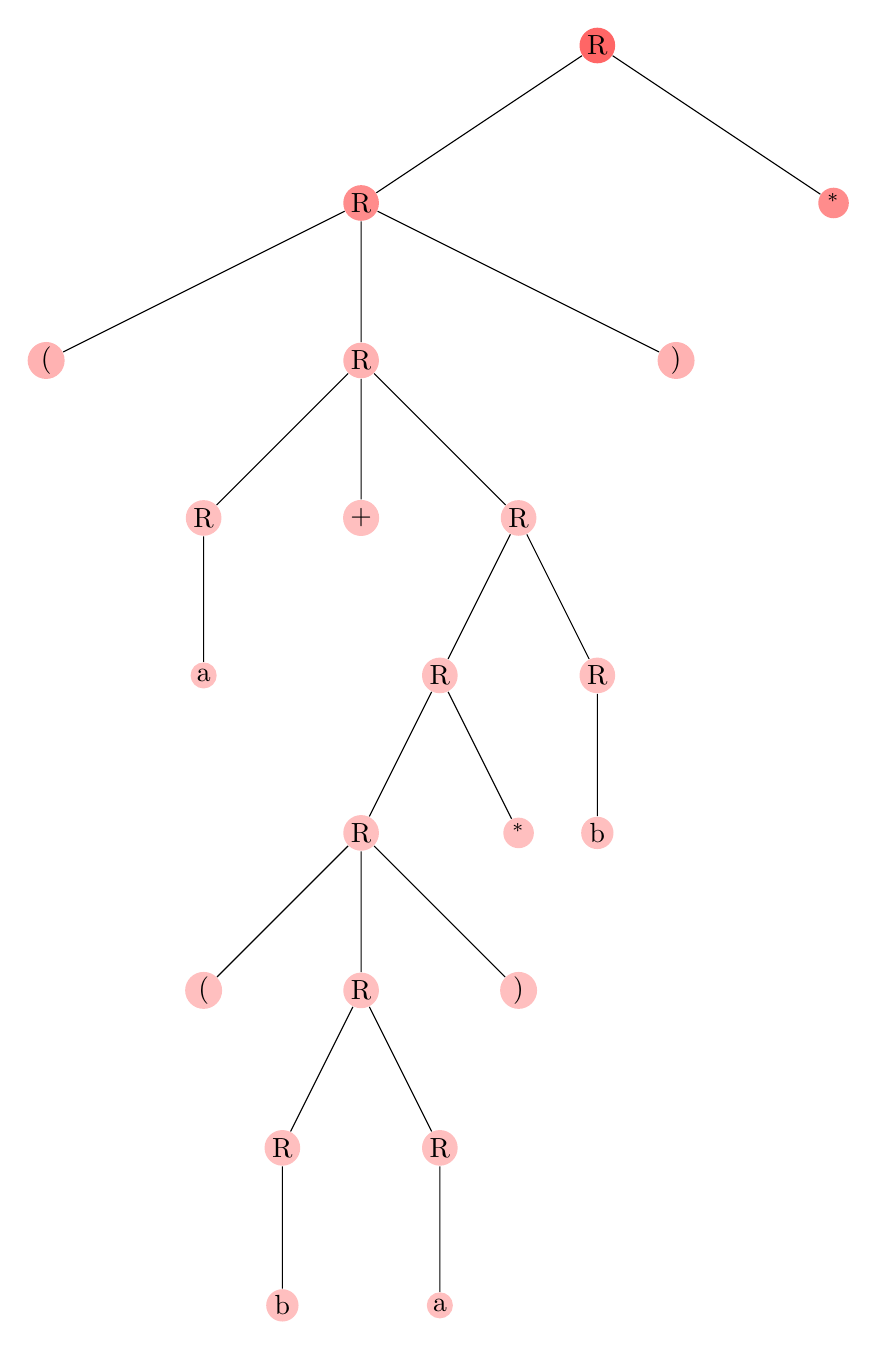
\begin{tikzpicture} [level distance=20mm,
                                every node/.style={fill=red!60,circle,inner sep=1pt},
                      level 1/.style={sibling distance=60mm,nodes={fill=red!45}}, level 2/.style={sibling distance=40mm,nodes={fill=red!30}}, level 3/.style={sibling distance=20mm,nodes={fill=red!25}}]
                \node {R} 
                  child {node{R}
                      child {node{$($}}
                      child {node{R}
                          child {node{R}
                              child {node{a}}
                          }
                          child {node{$+$}}
                          child {node{R}
                              child {node{R}
                                  child {node{R}
                                      child {node{$($}}
                                      child {node{R}
                                          child {node{R}
                                              child {node{b}}
                                          }
                                          child {node{R}
                                              child {node{a}}
                                          }
                                      }
                                      child {node{$)$}}
                                  }
                                  child {node{$^\ast$}}
                              }
                              child {node{R}
                                  child {node{b}}
                              }
                          }
                      }
                      child {node{$)$}}
                  }
                  child {node{$^\ast$}};

            \end{tikzpicture}
\end{enumerate}
  


   \newpage
   
\item \pts{$3\times 3= 9$} Consider the following CFG.
\[\begin{array}{cll}
S & \rightarrow & AED \mid F \\
A & \rightarrow & Aa \mid a \\
B & \rightarrow & Bb \mid b \\
C & \rightarrow & Cc \mid c \\
D & \rightarrow & Dd \mid d \\
E & \rightarrow & bEc \mid bc \\
F & \rightarrow & aFd \mid BC

\end{array}\]

\begin{enumerate}
\item What is the language generated by this grammar?
            \[\begin{array}{cll}
            S & \rightarrow & a^+b^mc^md^+ \mid a^nb^+c^+d^n  (m>=1,n>=0) \\
            %% Your answer here
            \end{array}\] 
\item Is the grammar as given ambiguous? If yes, give an example of an expression
with two parse trees under this grammar. If not, explain why that is the case. 
            \\
            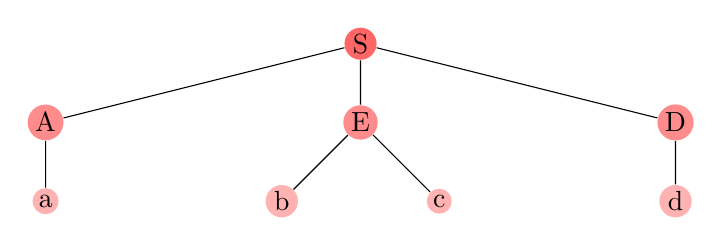
\begin{tikzpicture} [level distance=10mm,
                                every node/.style={fill=red!60,circle,inner sep=1pt},
                      level 1/.style={sibling distance=40mm,nodes={fill=red!45}}, level 2/.style={sibling distance=20mm,nodes={fill=red!30}}, level 3/.style={sibling distance=10mm,nodes={fill=red!25}}]
                \node {S} 
                  child{node{A}
                    child{node{a}}
                  }
                  child{node{E}
                    child{node{b}}
                    child{node{c}}
                  }
                  child{node{D}
                    child{node{d}}
                  };
            \end{tikzpicture}
            \\
            \\
            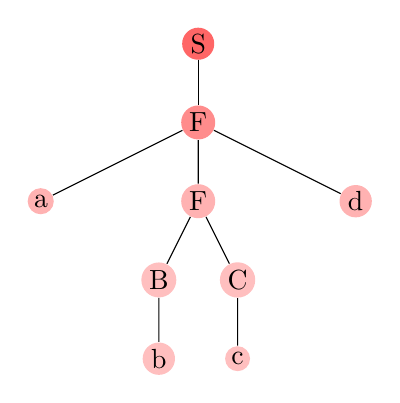
\begin{tikzpicture} [level distance=10mm,
                                every node/.style={fill=red!60,circle,inner sep=1pt},
                      level 1/.style={sibling distance=40mm,nodes={fill=red!45}}, level 2/.style={sibling distance=20mm,nodes={fill=red!30}}, level 3/.style={sibling distance=10mm,nodes={fill=red!25}}]
                \node {S} 
                  child {node{F}
                    child {node{a}}
                    child {node{F}
                      child {node{B}
                        child {node{b}}
                      }
                      child {node{C}
                        child {node{c}}
                      }
                    }
                    child {node{d}}
                  };
            \end{tikzpicture}
            \\
\item Transform the CFG given above by eliminating ambiguity and
left recursion, if needed.
            \[\begin{array}{cll}
                S & \rightarrow & AG \mid GD \mid F \\
                A & \rightarrow & Aa \mid a \\
                B & \rightarrow & Bb \mid b \\
                C & \rightarrow & Cc \mid c \\
                D & \rightarrow & Dd \mid d \\
                E & \rightarrow & bEc \mid bc \\
                F & \rightarrow & aFd \mid BC \\
                G & \rightarrow & aGd \mid E \\
            \end{array}\]
\end{enumerate}


   \newpage
\item \pts{$3\times 3= 9$} Consider the following CFG.
\[\begin{array}{cll}
A & \rightarrow & [AB] \mid a \\
B & \rightarrow & \epsilon \mid +AC \mid Cb \\
C & \rightarrow & \epsilon \mid -ABc
\end{array}\]

\begin{enumerate}
  \item Compute the First and Follow sets for the grammar.
             \[\begin{array}{cll}
              FIRST(A)=\{[\} \\
              FIRST(B)=\{\epsilon,+,-\} \\
              FIRST(C)=\{\epsilon,-\} \\
              FIRST(a)=\{a\} \\
              FIRST([AB])=\{[\} \\
              FIRST(+AC)=\{+\} \\
              FIRST(Cb)=\{\epsilon,-\} \\
              FIRST(-ABc)=\{-\} \\ \\
              FOLLOW(A)=\{+,-,],b,c,\$\} \\
              FOLLOW(B)=\{c,]\} \\
              FOLLOW(C)=\{b,c,]\} \\
            \end{array}\]
  \item Give the LL(1) parsing table for the grammar.
             \[\begin{array}{cll}
                 \begin{tabular}{|c|*{8}{c}|}
                        \hline
                        \diagbox{NT}{T} & a & b & c & + & - & [ & ] & \$ \\
                        \hline
                                      A & $A \rightarrow a$ &  &  &  & & $A \rightarrow [AB]$ & & \\
                        \hline
                                      B &  &  & $B \rightarrow \epsilon$ & $B \rightarrow +AC$ & $B \rightarrow Cb$ & & $B \rightarrow \epsilon$ & \\
                        \hline
                                      B &  &  & $B \rightarrow Cb$ &  &  &  & $B \rightarrow Cb$ & \\
                        \hline
                                      C &  & $C \rightarrow \epsilon$ & $C \rightarrow \epsilon$ &  & $C \rightarrow -ABc$ & & $C \rightarrow \epsilon$ & \\
                        \hline
                  \end{tabular}
            \end{array}\]
  \item Is this grammar LL(1)? and Why.
              \[\begin{array}{cll}
            NO,there \  are \  multiple \ choice \ in \  the \ B \  and \  c.
            \end{array}\]
\end{enumerate}

\item \pts{$8$}  Using the context-free grammar for Cool given in Section 11 of the Cool
manual, draw a parse tree for the following expression.
  \begin{lstlisting} 
    while not (x <-z <- 0) loop 
      y <- z + 2 * x + 1
    pool
  \end{lstlisting}
Note that the context-free grammar by itself is ambiguous, so you will
need to use the precedence and associativity rules in Section 11.1 to
get the correct tree.
            \\
            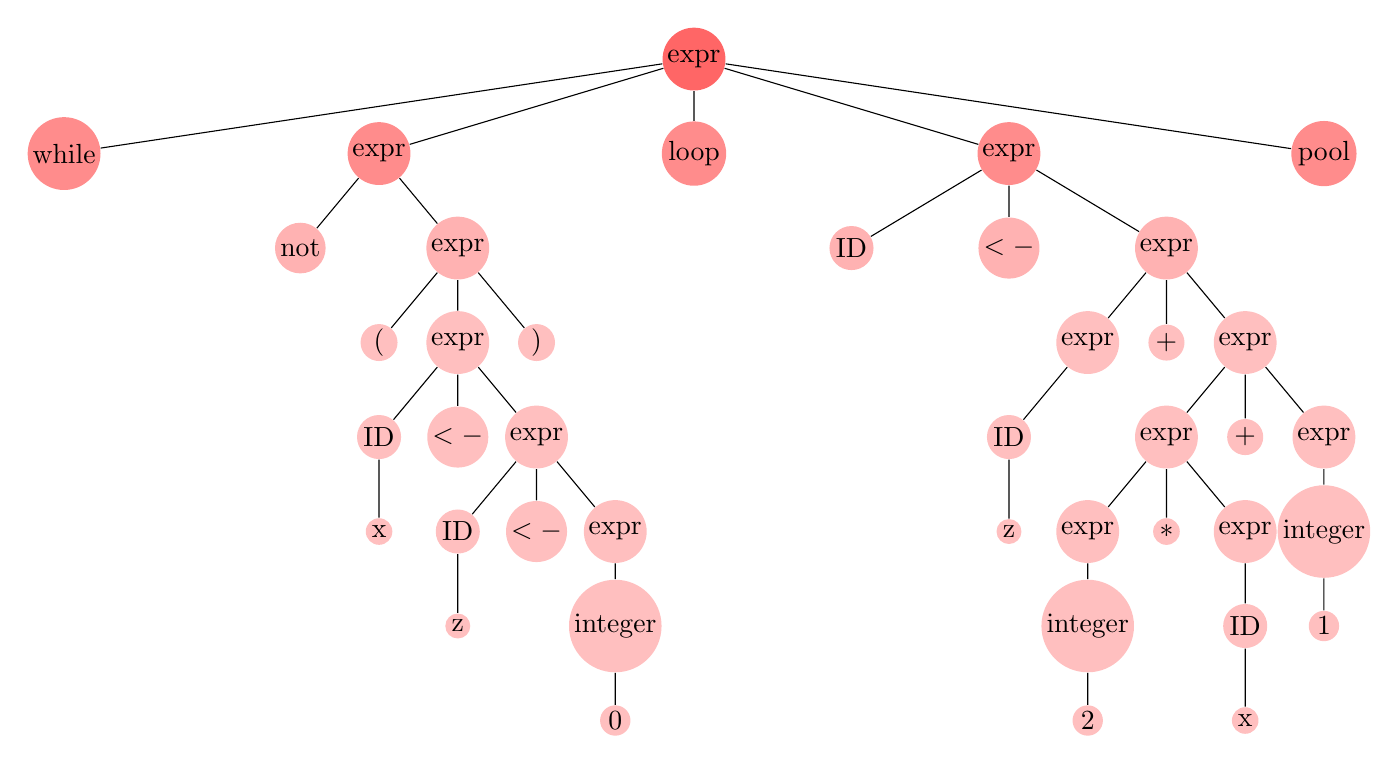
\begin{tikzpicture} [level distance=12mm,
                                every node/.style={fill=red!60,circle,inner sep=1pt},
                      level 1/.style={sibling distance=40mm,nodes={fill=red!45}}, level 2/.style={sibling distance=20mm,nodes={fill=red!30}}, level 3/.style={sibling distance=10mm,nodes={fill=red!25}}]
                \node {expr} 
                    child {node{while}}
                    child {node{expr}
                        child {node{not}}
                        child {node{expr}
                            child {node{$($}}
                            child {node{expr}
                                child {node{ID}
                                    child {node{x}}
                                }
                                child {node{$<-$}}
                                child {node{expr}
                                    child {node{ID}
                                        child {node{z}}
                                    }
                                    child {node{$<-$}}
                                    child {node{expr}
                                        child {node{integer}
                                            child {node{0}}
                                        }
                                    }
                                }
                            }
                            child {node{$)$}}
                        }
                    }
                    child {node{loop}}
                    child {node{expr}
                        child {node{ID}}
                        child {node{$<-$}}
                        child {node{expr}
                            child {node{expr}
                                child {node{ID}
                                    child {node{z}}
                                }
                                child [missing]
                                child [missing]
                            }
                            child {node{$+$}}
                            child {node{expr}
                                child {node{expr}
                                   child {node{expr}
                                      child {node{integer}
                                          child {node{2}}
                                      }
                                   }
                                   child {node{$*$}}
                                   child {node{expr}
                                      child {node{ID}
                                          child {node{x}}
                                      }
                                   }
                                }
                                child {node{$+$}}
                                child {node{expr}
                                    child {node{integer}
                                      child {node{1}}
                                    }
                                }
                            }
                        }
                    }
                    child {node{pool}};
            \end{tikzpicture}
            \\ 

\newpage
\item \pts{$4\times 4 =16$} Consider the following grammar describing a certain sort of nested lists:
\[\begin{array}{cll}
S & \rightarrow & T;S \mid \epsilon \\
T & \rightarrow & U\star T \mid U \\
U & \rightarrow & x\mid y\mid [S]  
\end{array}\]
$S$, $T$, and $U$ are nonterminals, while others are terminals.
\begin{enumerate}
  \item Left-factor this grammar.
             \[\begin{array}{cll}
                S & \rightarrow & T;S \mid \epsilon \\
                T & \rightarrow & UU' \\
                U' & \rightarrow & \star T \mid \epsilon \\
                U & \rightarrow & x\mid y\mid [S]  
            \end{array}\]
  \item Give the First and Follow sets for each nonterminal in the grammar obtained in part (a).
            \[\begin{array}{cll}
              FIRST(U)=\{x,y,[\} \\
              FIRST(T)=\{x,y,[\} \\
              FIRST(U')=\{\epsilon,\star\} \\
              FIRST(S)=\{x,y,[,\epsilon\} \\
              FIRST(T;S)=\{x,y,[\} \\
              FIRST(UU')=\{\epsilon,\star\} \\
              FIRST(\star T)=\{\star\} \\
              FIRST(x)=\{x\} \\ 
              FIRST(y)=\{y\} \\ 
              FIRST([S])=\{[\} \\ \\ 
              FOLLOW(S)=\{],\$\} \\
              FOLLOW(T)=\{;\} \\
              FOLLOW(U)=\{\star,;\} \\
              FOLLOW(U')=\{;\} \\
            \end{array}\]
  \item Using this information, construct an LL(1) parsing table for the grammar obtained in part (a).
             \[\begin{array}{cll}
                 \begin{tabular}{|c|*{7}{c}|}
                        \hline
                        \diagbox{NT}{T} & x & y & ; & $\star$ & [ & ] & \$ \\
                        \hline
                                      S & $S \rightarrow T;S$ & $S \rightarrow T;S$ &  &  & $S \rightarrow T;S$ & $S \rightarrow \epsilon $ & $S \rightarrow \epsilon $ \\
                        \hline
                                      T &  &  & $T \rightarrow UU'$ & $T \rightarrow UU'$  &  & & \\
                        \hline
                                      U' &  &  & $U' \rightarrow \epsilon $ & $U' \rightarrow \star T$ &  & & \\
                        \hline
                                      U & $U \rightarrow x$ & $U \rightarrow y$ &  &  & $U \rightarrow [S]$ & & \\
                        \hline
                  \end{tabular}
            \end{array}\]
  \item Suppose we generated an LL(1) parser for the grammar using the table you constructed. What would go wrong if it tried to parse the following input string?
  \[[x;y]\star [;\]
            \[\begin{array}{cll}
            %% Your answer here
                    S & \rightarrow T;S \\
                      & \rightarrow UU';S \\
                      & \rightarrow [S]U';S \\
                      & \rightarrow [T;S]U';S \\
                      & \rightarrow [UU';S]U';S \\
                      & \rightarrow [xU';S]U';S \\
                      & \rightarrow [xU';S]U';S \\
                      & \rightarrow [x;S]U';S \\
                      & \rightarrow [x;T;S]U';S \  \ here \ is \ wrong \ S \rightarrow T;S \\

            \end{array}\] 
\end{enumerate}

\newpage
\item \pts{$3\times 2+5\times 2 =16$} Consider the following CFG, which has the set of terminals
$T = \{ \textbf{a}, \textbf{b} \}$.
\[\begin{array}{cll}
 S & \rightarrow & X \textbf{a} \\
X & \rightarrow & \textbf{a} \mid \textbf{a} X \textbf{b} 
\end{array}\]
 
\begin{enumerate}

\item Construct a DFA for viable prefixes of this grammar using LR(0)
items.
          \[\begin{array}{cll}
            %% Your answer here
              let \ q(1) = & S' & \rightarrow .S \\
                           & S & \rightarrow .Xa \\
                           & X & \rightarrow .a \\
                           & X & \rightarrow .aXb \\
                           \\
              let \ q(2) = & X & \rightarrow a. \\
                           & X & \rightarrow a.Xb \\
                           & X & \rightarrow .a \\
                           & X & \rightarrow .aXb \\
                           \\
              let \ q(3) = & S' & \rightarrow S. \\
                           \\
              let \ q(4) = & S & \rightarrow X.a \\
                           \\
              let \ q(5) = & X & \rightarrow aX.b \\
                           \\
              let \ q(6) = & S & \rightarrow Xa. \\
                           \\
              let \ q(7) = & X & \rightarrow aXb. \\
                           \\
              let \ q(8) = & &accept \\
           \end{array}\] 
            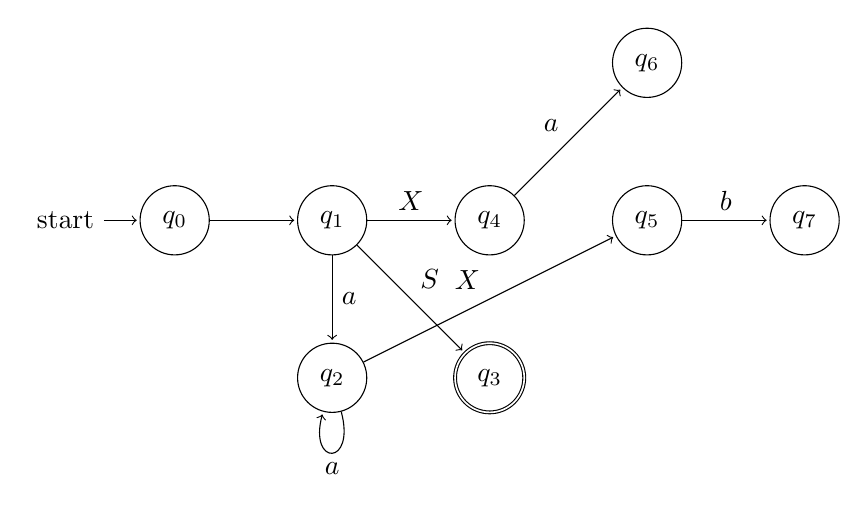
\begin{tikzpicture}[shorten >=1pt,node distance=2cm,on grid,auto]
                    \node[state,initial]   (q_0)   {$q_0$};
                    \node[state]   (q_1) [right=of q_0]  {$q_1$};
                    \node[state]   (q_2) [below=of q_1]  {$q_2$};
                    \node[state,accepting]   (q_3) [right=of q_2]  {$q_3$};
                    \node[state]   (q_4) [above=of q_3]  {$q_4$};
                    \node[state]   (q_5) [right=of q_4]  {$q_5$};
                    \node[state]   (q_6) [above=of q_5]  {$q_6$};
                    \node[state]   (q_7) [right=of q_5]  {$q_7$};
                    \path[->]
                    (q_0) edge node {} (q_1)
                    (q_1) edge node {$a$} (q_2) 
                          edge node {$S$} (q_3) 
                          edge node {$X$} (q_4) 
                    (q_2) edge [loop below] node {$a$} (q_2) 
                          edge node {$X$} (q_5) 
                    (q_4) edge node {$a$} (q_6) 
                    (q_5) edge node {$b$} (q_7);
              
            \end{tikzpicture}
\item Identify a shift-reduce conflict in this grammar under the
SLR(1) rules.
          \[\begin{array}{cll}
                shift-reduce \  conflict
                 \begin{tabular}{|c|*{6}{c}|}
                        \hline
                        \diagbox{state}{T} & S & x & a & b & \$ & action S \\
                        \hline
                                      1 & s3 & s4 & s2 & & & 3 \\
                        \hline
                                      2 &  & s5 & s2 & & & \\
                                        & r2 & r2 & r2 & r2 & r2 & \\
                        \hline
                                      3 & & & & &  acc & \\
                        \hline
                                      4 & & & s6 & & & \\
                        \hline
                                      5 & & & & s7 & & \\
                        \hline
                                      6 & r6 & r6 & r6 & r6 & r6  & \\
                        \hline
                                      7 & r7 & r7 & r7 & r7 & r7  & \\

                        
                        \hline
                  \end{tabular}
            \end{array}\]
\item Assuming that an SLR(1) parser resolves shift-reduce conflicts
by choosing to shift, show the operation of such a parser on the input
string \textbf{aaba}.
          \[\begin{array}{cll}
            %% Your answer here
                    S & \rightarrow Xa \\
                      & \rightarrow aXba \\
                      & \rightarrow aaba \\
            \end{array}\] 
\item Suppose that the production $X \rightarrow \varepsilon$ is added
to this grammar.  Identify a reduce-reduce conflict in the resulting
grammar under the SLR(1) rules.
           \[\begin{array}{cll}
                 reduce-reduce \  conflict
            \end{array}\]
\end{enumerate}
\end{enumerate}
\end{document}

